The equation of the line is 
%
\begin{align}
\vec{x} &= \vec{A}+\lambda\brak{\vec{B}-\vec{A}}
\end{align}
The equation of the plane can be represented as 
\begin{align}
    \vec{n}^T\vec{x}=c
\end{align}
The point of intersection of the line and the plane satisfies the plane equation and is given by
\begin{align}
    c&=\vec{n}^T(\vec{x})\\
    &=\vec{n}^T(\vec{A}+\lambda\brak{\vec{B}-\vec{A}})
\end{align}  
Thus,
\begin{align}   
\lambda=\frac{c-\vec{n}^T\vec{A}}{\vec{n}^T(\vec{B}-\vec{A})}
\end{align}
The point of intersection is then given by
\begin{align}
    \vec{x}=\vec{A}+\brak{\frac{c-\vec{n}^T\vec{A}}{\vec{n}^T(\vec{B}-\vec{A})}}\brak{\vec{B}-\vec{A}}
\end{align}
For the given problem,
\begin{align}
\vec{A}&= \myvec{5\\1\\6} \\
\vec{B}&= \myvec{2\\-3\\5}\\
\vec{n}&=\myvec{1\\0\\0}\\
    c&=0
\end{align}
Solving the above we get
\begin{align}
    \lambda=\frac{-5}{2}
\end{align}
Substituting the value of $\lambda$ we have the point of contact as
\begin{align}
 \vec{x}=\myvec{5\\1\\6} -\frac{5}{2}\myvec{2\\-3\\5} = \frac{1}{2}\myvec{0\\17\\-13}
\end{align}
See fig. \ref{aug/2/26/fig:Line }	.
\begin{figure}[!ht]
\centering
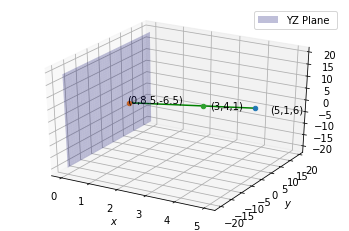
\includegraphics[ width=\columnwidth]{solutions/aug/2/36/figures/plot.png}
\caption{Line and point of intersection}
\label{aug/2/26/fig:Line }	
\end{figure}

